\paragraph{本机可复核证据与历史记录分开。}
旧 CPU 工件按研究决策不再保留，旧 $10/10$、$50/50$、UR5e 与移动身体
数字已移入不参与本文编译的历史文件，不能作为当前论文结果。当前证据以本机
保存的原始轨迹、计费账本、源码与环境快照为准。所有下述结果均为开发研究，
不代替正式工业任务、真实机器人或总体统计。

\paragraph{P1：校准有效性与候选可行性分离。}
冻结本机重新生成的 Panda reference prior；xArm7 的 matched 为
gain $1$/delay $0$，derated 为 gain $0.65$/delay $60\,\mathrm{ms}$。
matched 仅指两个执行器参数，不能理解为两个身体具有相同闭环响应。
每条件三次独立校准/优化，每次五个探针，三条拟合、两条独立验证。
所有六次响应验证通过；每次 calibrated/nominal 分别使用
$12\times2\times2=48$ 条模型搜索轨迹，full 与 task-only 共享同一池。
四方法共 $240$ 条实际目标评估独立重算为零判定不一致。
\begin{center}
\small
\begin{tabular}{lrrrr}
\toprule
xArm7 条件 & Direct & Calibrated map & Same-model task-only & Nominal response\\
\midrule
Derated & 0/30 & 29/30 & 29/30 & 8/30\\
Matched & 0/30 & 3/30 & 3/30 & 3/30\\
\bottomrule
\end{tabular}
\end{center}
六次优化 full/task-only 均选同一映射；所有方法每条件的模式标签均
$30/30$，包括失败轨迹，因此标签保持不能代替可执行模式覆盖。
这批数据支持受控结构族中 derated 条件的校准效用，未建立 response
anchoring 相对同模型控制优化的增量。

\paragraph{P1.5：已有轨迹的失败诊断。}
已有 $240$ 对实际/校准模型轨迹的终止状态与时间全部一致。
matched 的 calibrated map 有 $17$ 次轴向支撑丢失、$10$ 次超时和
$3$ 次成功。前者使用约 $5\,\mathrm N$ 的 transported 命令，
接触后法向力降至零；超时组使用约 $12.5\,\mathrm N$ 命令，
最终实际力约 $10.10$--$10.83\,\mathrm N$，任务要求仍为
$5\pm2.5\,\mathrm N$。三条成功在保持窗口中最小力裕度只有
$0.0008$--$0.0144\,\mathrm N$。derated 的唯一失败为侧向力
$17.30\,\mathrm N>10\,\mathrm N$，总力约 $22.01\,\mathrm N<25\,\mathrm N$。
matched 的力矩比峰值小于 $0.534$，未见执行器力矩饱和证据；积分限幅
是另一事实。四条另行计账的开发复现均重现原终止状态，并记录接触 witness、
接触记忆、积分和 hold/loss 计数。诊断准确不排除公共控制或物理实现缺陷。

\begin{figure}[htbp]
\centering
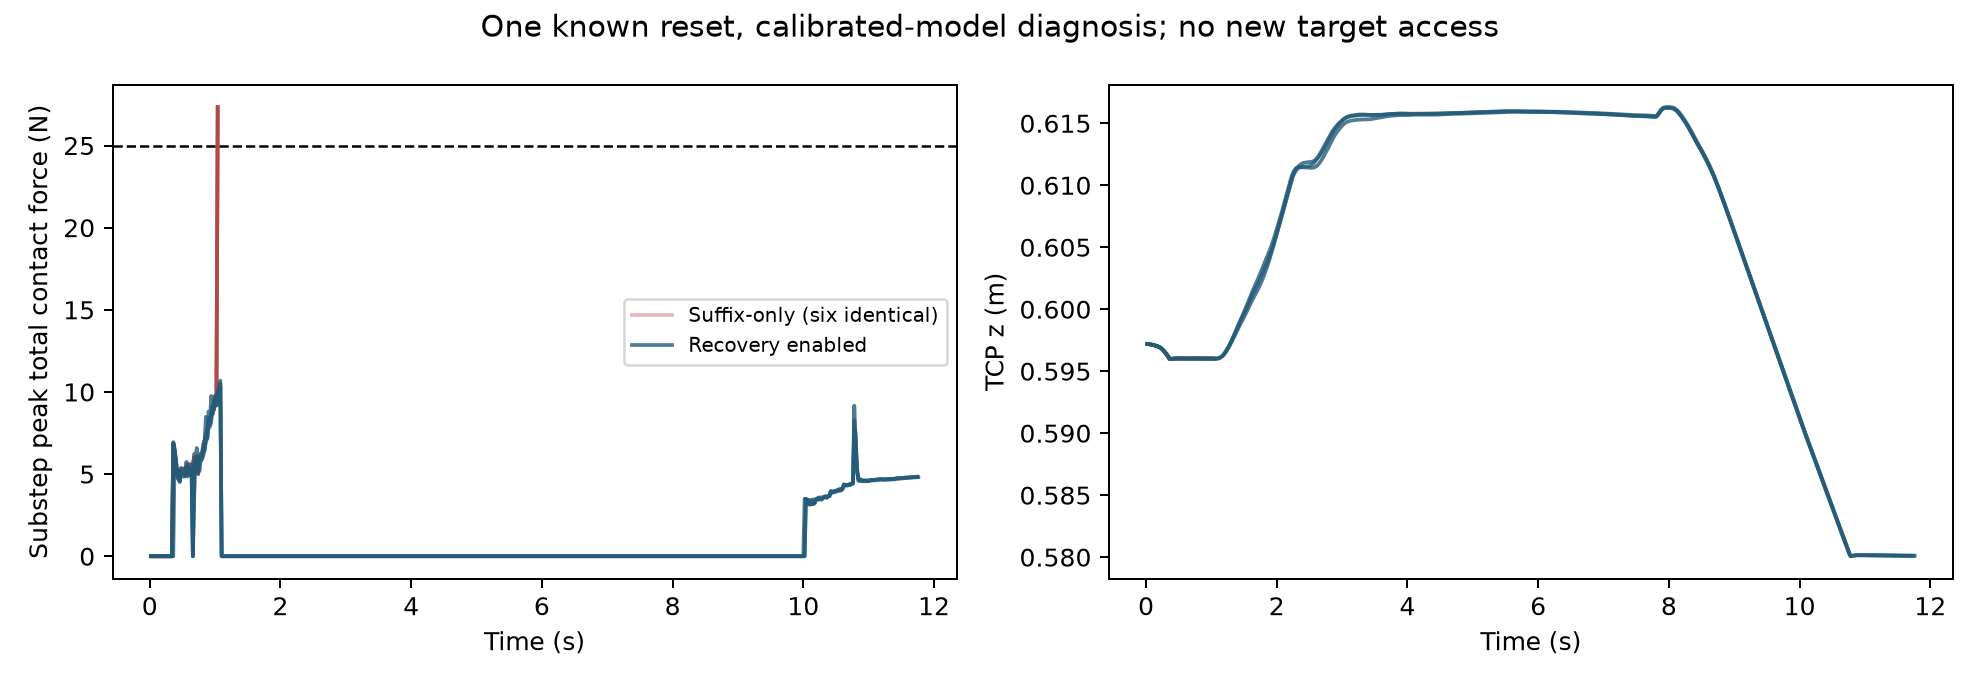
\includegraphics[width=.94\linewidth]{figures/prefix_diagnosis.png}
\caption{单个已知开发 reset 的 calibrated-model 配对诊断。六个仅修改后缀的
候选在相同前缀上超力；图中三个恢复 profile 的代表轨迹完成任务。
完整诊断为六个控制失败、十八个回撤补偿成功，未新增目标访问，不是总体因果证书。}
\end{figure}

\paragraph{P1.6：预先固定的可行映射实验。}
保持几何、控制器、任务期限与力限不变，固定 $24$ 个候选：保留原
$12$ 个阶段映射，增加 $1.25/1.5/1.75/2$ 的中间力倍率，并加入有限
正负全阶段阻抗补偿。每次新校准各五探针，calibrated 与 nominal
各 $24\times4\times2=192$ 条训练模型轨迹；full/task-only 共享全部
候选、条件与缓冲。先要求有限训练 reset 中两模式均成功，再于
task-only 最小任务成本的 $\delta=0.02$ 带内最小化归一化响应差异。
另用四个模型验证 reset 过滤；全失败时返回
\texttt{no\_feasible\_candidate}，不强行部署最少失败的候选。
之后冻结映射，在每重复五个新 reset、两模式上评价；重复为
$7100/8100/9100$，旧开发 reset 不进入本次评估。
% Generated from independently audited scientific_report.json.
\begin{center}\small
\begin{tabular}{lrr}
\toprule
Method & Derated & Matched\\
\midrule
Direct & 0/30 & 1/30\\
Full & 27/30 & 10/30\\
Task-only & 27/30 & 10/30\\
Nominal & 1/30 & 10/30\\
\bottomrule
\end{tabular}
\end{center}
本阶段新探针 30 次，实际不同目标评估 120 条；别名方法与拒绝另报。


\paragraph{恢复支持的单列 v2。}
v1 两个 matched 校准格拒绝候选，不能只报已部署一格的 $10/10$。
根据开发模型中阶段 $1$ 的超力，v2 保留六个代表候选，并加入三种
有界恢复阻抗 profile、三种终段力倍率与两种阶段刚度，共 $24$ 个。
恢复、对齐、插入的刚度独立，终段力倍率不放大初始加载。
使用相同六份已计费校准，新增探针为零，全部 reset 增加
$50{,}000{,}000$；共同控制器、力限与时限保持。
这是基于 v1 开发信息设计的第二个开发协议，不是未见机制确认性实验。
% Generated from independently audited scientific_report.json.
\begin{center}\small
\begin{tabular}{lrr}
\toprule
Method & Derated & Matched\\
\midrule
Direct & 0/30 & 0/30\\
Full & 20/30 & 30/30\\
Task-only & 20/30 & 30/30\\
Nominal & 9/30 & 30/30\\
\bottomrule
\end{tabular}
\end{center}
本阶段新探针 0 次，实际不同目标评估 170 条；别名方法与拒绝另报。

v2 matched 三个重复均 $10/10$；derated 两个重复各 $10/10$，另一个
因独立模型验证失败拒绝，故总体是 $20/30$，不能只报告已部署的全成功。
完整方法与 task-only 的任务成功数相同；名义模型在 matched 也为 $30/30$。

同一映射、reset 与随机流的重复方法名称合并为一次物理执行，逻辑方法
分母和实际不同执行次数分列。全部拒绝仍进入请求分母。零模型误差、全成功
或经验过滤均不认证无限策略类 uniform bound。详细路径、账本和统计单位见
\url{docs/development/cross-embodiment-p1-refinement.md}。
